\vspace{-0.3em}
\section{Experimental Evaluation}
\vspace{-0.4em}


The purpose of our experiments is to evaluate the effectiveness of RL algorithms for finetuning diffusion models to align with a variety of user-specified objectives.
After examining the viability of the general approach, we focus on the following questions:

\vspace{-0.3em}
\begin{enumerate}
    \item How do variants of \methodours{} compare to \methodrwr{} and to each other?
    \item Can VLMs allow for optimizing rewards that are difficult to specify manually?
    \item Do the effects of RL finetuning generalize to prompts not seen during finetuning?
\end{enumerate}

\subsection{Algorithm Comparisons}
\label{sec:alg_comparison}

We begin by evaluating all methods on the compressibility, incompressibility, and aesthetic quality tasks, as these tasks isolate the effectiveness of the RL approach from considerations relating to the VLM reward function.
We use Stable Diffusion v1.4 \citep{rombach2022latent} as the base model for all experiments.
Compressibility and incompressibility prompts are sampled uniformly from all 398 animals in the ImageNet-1000 \citep{deng2009imagenet} categories.
Aesthetic quality prompts are sampled uniformly from a smaller set of 45 common animals.

\begin{figure}
    \centering
    \begin{minipage}{0.48\linewidth}
        \begin{centering}
            \footnotesize 
            \textbf{Pretrained} \\
            \vspace{0.5em}
        \end{centering}
        \lfbox[
            border-width=2pt,
            padding-top=0pt,
            padding-bottom=0pt,
            padding-left=-2.5pt,
            padding-right=-8.5pt,
        ]{
            \begin{minipage}{\linewidth}
                \includegraphics*[width=0.25\linewidth]{algorithm-comparison/lora/pretrained/fox.jpg}
                \hspace{-0.7em}
                \includegraphics*[width=0.25\linewidth]{algorithm-comparison/lora/pretrained/dolphin.jpg}
                \hspace{-0.7em}
                \includegraphics*[width=0.25\linewidth]{algorithm-comparison/lora/pretrained/cow.jpg}
                \hspace{-0.7em}
                \includegraphics*[width=0.25\linewidth]{algorithm-comparison/lora/pretrained/hedgehog.jpg} \\
                \vspace{-1.25em} \\
                \includegraphics*[width=0.25\linewidth]{algorithm-comparison/lora/pretrained/wolf.jpg}
                \hspace{-0.7em}
                \includegraphics*[width=0.25\linewidth]{algorithm-comparison/lora/pretrained/horse.jpg}
                \hspace{-0.7em}
                \includegraphics*[width=0.25\linewidth]{algorithm-comparison/lora/pretrained/pig.jpg}
                \hspace{-0.7em}
                \includegraphics*[width=0.25\linewidth]{algorithm-comparison/lora/pretrained/squirrel.jpg}
            \end{minipage}
        }
    \end{minipage}
    \hfill
    \begin{minipage}{0.48\linewidth}
        \begin{centering}
            \footnotesize 
            \textbf{Aesthetic Quality} \\
            \vspace{0.5em}
        \end{centering}
        \lfbox[
            border-width=2pt,
            padding-top=0pt,
            padding-bottom=0pt,
            padding-left=-2.5pt,
            padding-right=-8.5pt,
        ]{
            \begin{minipage}{\linewidth}
                \includegraphics*[width=0.25\linewidth]{algorithm-comparison/lora/aesthetic/fox.jpg}
                \hspace{-0.7em}
                \includegraphics*[width=0.25\linewidth]{algorithm-comparison/lora/aesthetic/dolphin.jpg}
                \hspace{-0.7em}
                \includegraphics*[width=0.25\linewidth]{algorithm-comparison/lora/aesthetic/cow.jpg}
                \hspace{-0.7em}
                \includegraphics*[width=0.25\linewidth]{algorithm-comparison/lora/aesthetic/hedgehog.jpg} \\
                \vspace{-1.25em} \\
                \includegraphics*[width=0.25\linewidth]{algorithm-comparison/lora/aesthetic/wolf.jpg}
                \hspace{-0.7em}
                \includegraphics*[width=0.25\linewidth]{algorithm-comparison/lora/aesthetic/horse.jpg}
                \hspace{-0.7em}
                \includegraphics*[width=0.25\linewidth]{algorithm-comparison/lora/aesthetic/pig.jpg}
                \hspace{-0.7em}
                \includegraphics*[width=0.25\linewidth]{algorithm-comparison/lora/aesthetic/squirrel.jpg}
            \end{minipage}
        }
    \end{minipage}
    \vspace{0.5em}\\
    \begin{minipage}{0.48\linewidth}
        \begin{centering}
            \footnotesize 
            \textbf{Compressibility} \\
            \vspace{0.5em}
        \end{centering}
        \lfbox[
            border-width=2pt,
            padding-top=0pt,
            padding-bottom=0pt,
            padding-left=-2.5pt,
            padding-right=-8.5pt,
        ]{
            \begin{minipage}{\linewidth}
                \includegraphics*[width=0.25\linewidth]{algorithm-comparison/lora/compress/fox.jpg}
                \hspace{-0.7em}
                \includegraphics*[width=0.25\linewidth]{algorithm-comparison/lora/compress/dolphin.jpg}
                \hspace{-0.7em}
                \includegraphics*[width=0.25\linewidth]{algorithm-comparison/lora/compress/cow.jpg}
                \hspace{-0.7em}
                \includegraphics*[width=0.25\linewidth]{algorithm-comparison/lora/compress/hedgehog.jpg} \\
                \vspace{-1.25em} \\
                \includegraphics*[width=0.25\linewidth]{algorithm-comparison/lora/compress/wolf.jpg}
                \hspace{-0.7em}
                \includegraphics*[width=0.25\linewidth]{algorithm-comparison/lora/compress/horse.jpg}
                \hspace{-0.7em}
                \includegraphics*[width=0.25\linewidth]{algorithm-comparison/lora/compress/pig.jpg}
                \hspace{-0.7em}
                \includegraphics*[width=0.25\linewidth]{algorithm-comparison/lora/compress/squirrel.jpg}
            \end{minipage}
        }
    \end{minipage}
    \hfill
    \begin{minipage}{0.48\linewidth}
        \begin{centering}
            \footnotesize 
            \textbf{Incompressibility} \\
            \vspace{0.5em}
        \end{centering}
        \lfbox[
            border-width=2pt,
            padding-top=0pt,
            padding-bottom=0pt,
            padding-left=-2.5pt,
            padding-right=-8.5pt,
        ]{
            \begin{minipage}{\linewidth}
                \includegraphics*[width=0.25\linewidth]{algorithm-comparison/lora/incompress/fox.jpg}
                \hspace{-0.7em}
                \includegraphics*[width=0.25\linewidth]{algorithm-comparison/lora/incompress/dolphin.jpg}
                \hspace{-0.7em}
                \includegraphics*[width=0.25\linewidth]{algorithm-comparison/lora/incompress/cow.jpg}
                \hspace{-0.7em}
                \includegraphics*[width=0.25\linewidth]{algorithm-comparison/lora/incompress/hedgehog.jpg} \\
                \vspace{-1.25em} \\
                \includegraphics*[width=0.25\linewidth]{algorithm-comparison/lora/incompress/wolf.jpg}
                \hspace{-0.7em}
                \includegraphics*[width=0.25\linewidth]{algorithm-comparison/lora/incompress/horse.jpg}
                \hspace{-0.7em}
                \includegraphics*[width=0.25\linewidth]{algorithm-comparison/lora/incompress/pig.jpg}
                \hspace{-0.7em}
                \includegraphics*[width=0.25\linewidth]{algorithm-comparison/lora/incompress/squirrel.jpg}
            \end{minipage}
        }
    \end{minipage} \\
    \caption{
        \textbf{(\methodours{} samples)}
        Qualitative depiction of the effects of RL finetuning on different reward functions.
        \methodours{} transforms naturalistic images into stylized artwork to maximize aesthetic quality, removes background content and applies foreground smoothing to maximize compressibility, and adds high-frequency noise to maximize incompressibility.
    }
    \label{fig:alg_samples}
    \vspace{-0.5em}
\end{figure}


\begin{figure}[t]
    \centering
    
\includegraphics[width=\linewidth]{algorithms_new.pdf}
    {\color{white}\rule{2.25em}{1em}}
    \raisebox{0.14em}{\color{ppo}\rule{1.5em}{0.15em}}
        ~\methodppo{}
        \hspace{1.5em}
    \raisebox{0.14em}{\color{pg}\rule{1.5em}{0.15em}}
        ~\methodreinforce{}
        \hspace{1.5em}
    \raisebox{0.14em}{\color{rwr}\rule{1.5em}{0.15em}}
        ~\methodrwr{}
        \hspace{1,5em}
    \raisebox{0.14em}{\color{ff}\rule{1.5em}{0.15em}}
        ~\methodff{}
    {
    }
    \caption{
        \textbf{(Finetuning effectiveness)}
        The relative effectiveness of different RL algorithms on three reward functions.
        We find that the policy gradient variants, denoted \methodours{}, are more effective optimizers than both RWR variants.
    }
    \label{fig:alg_comparison}
    \vspace{-10pt}
\end{figure}


As shown qualitatively in Figure~\ref{fig:alg_samples}, \methodours{} is able to effectively adapt a pretrained model with only the specification of a reward function and without any further data curation.
The strategies found to optimize each reward are nontrivial; for example, to maximize LAION-predicted aesthetic quality, \methodours{} transforms a model that produces naturalistic images into one that produces artistic drawings.
To maximize compressibility, \methodours{} removes backgrounds and applies smoothing to what remains.
To maximize incompressibility, \methodours{} finds artifacts that are difficult for the JPEG compression algorithm to encode, such as high-frequency noise and sharp edges.
Samples from \methodrwr{} are provided in Appendix~\ref{app:more_samples} for comparison.

We provide a quantitative comparison of all methods in Figure~\ref{fig:alg_comparison}.
We plot the attained reward as a function of the number of queries to the reward function, as reward evaluation becomes the limiting factor in many practical applications.
\methodours{} shows a clear advantage over \methodrwr{} on all tasks, demonstrating that formulating the denoising process as a multi-step MDP and estimating the policy gradient directly is more effective than optimizing a reward-weighted variational bound on log-likelihood. Within the \methodours{} class, the importance sampling estimator slightly outperforms the score function estimator, likely due to the increased number of optimization steps. Within the \methodrwr{} class, the performance of weighting schemes is comparable, making the sparse weighting scheme preferable on these tasks due to its simplicity and reduced resource requirements.






\begin{figure}
    \centering
    \adjustbox{valign=t}{
        \begin{minipage}{0.68\linewidth}
            \begin{minipage}{\linewidth}
                {
                    \hspace{4em}
                    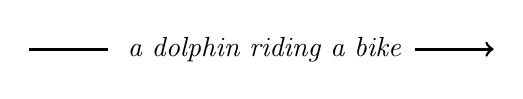
\begin{tikzpicture}
                        \draw[-, line width=1pt] (0,0) -- (1,0);
                        \node at (3,0) {\emph{a dolphin riding a bike}}; 
                        \draw[->, line width=1pt] (4.9,0) -- (5.9,0);
                    \end{tikzpicture} \\
                }
                \lfbox[
                    border-width=2pt,
                    padding-top=0pt,
                    padding-bottom=0pt,
                    padding-left=-2.6pt,
                    padding-right=-2.5pt,
                ]{
                    \includegraphics*[width=0.2\linewidth]{vlm/dolphin_bike/0.jpg}
                    \hspace{-0.7em}
                    
\includegraphics[width=0.2\linewidth]{vlm/dolphin_bike/1.jpg}
                    \hspace{-0.7em}
                    \includegraphics*[width=0.2\linewidth]{vlm/dolphin_bike/2.jpg}
                    \hspace{-0.7em}
                    \includegraphics*[width=0.2\linewidth]{vlm/dolphin_bike/3.jpg}
                    \hspace{-0.7em}
                    \includegraphics*[width=0.2\linewidth]{vlm/dolphin_bike/5.jpg}
                }
            \end{minipage}
            \vspace{0em} \\
            \begin{minipage}{\linewidth}
                {
                    \hspace{4em}
                    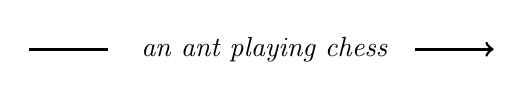
\begin{tikzpicture}
                        \draw[-, line width=1pt] (0,0) -- (1,0);
                        \node at (3,0) {\emph{an ant playing chess}}; 
                        \draw[->, line width=1pt] (4.9,0) -- (5.9,0);
                    \end{tikzpicture} \\
                }
                \lfbox[
                    border-width=2pt,
                    padding-top=0pt,
                    padding-bottom=0pt,
                    padding-left=-2.6pt,
                    padding-right=-2.5pt,
                ]{
                    \includegraphics*[width=0.2\linewidth]{vlm/ant_chess/0.jpg}
                    \hspace{-0.7em}
                    
\includegraphics[width=0.2\linewidth]{vlm/ant_chess/1.jpg}
                    \hspace{-0.7em}
                    \includegraphics*[width=0.2\linewidth]{vlm/ant_chess/3.jpg}
                    \hspace{-0.7em}
                    \includegraphics*[width=0.2\linewidth]{vlm/ant_chess/4.jpg}
                    \hspace{-0.7em}
                    \includegraphics*[width=0.2\linewidth]{vlm/ant_chess/5.jpg}
                }
            \end{minipage}
            \vspace{0em} \\
            \begin{minipage}{\linewidth}
                {
                    \hspace{4em}
                    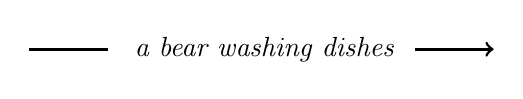
\begin{tikzpicture}
                        \draw[-, line width=1pt] (0,0) -- (1,0);
                        \node at (3,0) {\emph{a bear washing dishes}}; 
                        \draw[->, line width=1pt] (4.9,0) -- (5.9,0);
                    \end{tikzpicture} \\
                }
                \lfbox[
                    border-width=2pt,
                    padding-top=0pt,
                    padding-bottom=0pt,
                    padding-left=-2.6pt,
                    padding-right=-2.5pt,
                ]{
                    \includegraphics*[width=0.2\linewidth]{vlm/bear_dishes/0.jpg}
                    \hspace{-0.7em}
                    \includegraphics*[width=0.2\linewidth]{vlm/bear_dishes/2.jpg}
                    \hspace{-0.7em}
                    \includegraphics*[width=0.2\linewidth]{vlm/bear_dishes/3.jpg}
                    \hspace{-0.7em}
                    \includegraphics*[width=0.2\linewidth]{vlm/bear_dishes/4.jpg}
                    \hspace{-0.7em}
                    \includegraphics*[width=0.2\linewidth]{vlm/bear_dishes/5.jpg}
                }
            \end{minipage}
        \end{minipage}
    }
    \hspace{-0.5em}
    \adjustbox{valign=t}{
        \begin{minipage}{0.29\linewidth}
            ~\vspace{1.5em} \\
            
\includegraphics[width=\linewidth]{vlm/plot.pdf} \\
            \vspace{-0.5em}\\
            \footnotesize
            ~\hspace*{3em}\raisebox{0.2em}{\color{bike}\rule{1.5em}{0.15em}}
                ~\emph{\ldots riding a bike} \\
            ~\hspace*{3em}\raisebox{0.2em}{\color{chess}\rule{1.5em}{0.15em}}
                ~\emph{\ldots playing chess} \\
            ~\hspace*{3em}\raisebox{0.2em}{\color{dishes}\rule{1.5em}{0.15em}}
                ~\emph{\ldots washing dishes}
        \end{minipage}
    }
    \vspace{0.0em}\\
    \caption{
        \textbf{(Prompt alignment)}
        \textbf{(L)}
        Progression of samples for the same prompt and random seed over the course of training.
        The images become significantly more faithful to the prompt.
        The samples also adopt a cartoon-like style, which we hypothesize is because the prompts are more likely depicted as illustrations than realistic photographs in the pretraining distribution.
        \textbf{(R)}
        Quantitative improvement of prompt alignment.
        Each thick line is the average score for an activity, while the faint lines show average scores for a few randomly selected individual prompts.
    }
    \label{fig:vlm_progression}
    \vspace{-1.2em}
\end{figure}



\vspace{-5pt}
\subsection{Automated Prompt Alignment}
We next evaluate the ability of VLMs, in conjunction with DDPO, to automatically improve the image-prompt alignment of the pretrained model without additional human labels.
We focus on \methodppo{} for this experiment, as we found it to be the most effective algorithm in Section~\ref{sec:alg_comparison}.
The prompts for this task all have the form ``\emph{a(n) [animal] [activity] }'', where the animal comes from the same list of 45 common animals used in Section~\ref{sec:alg_comparison} and the activity is chosen from a list of 3 activities: ``\emph{riding a bike}'', ``\emph{playing chess}'', and ``\emph{washing dishes}''. 

The progression of finetuning is depicted in Figure~\ref{fig:vlm_progression}.
Qualitatively, the samples come to depict the prompts much more faithfully throughout the course of training.
This trend is also reflected quantitatively, though is less salient as small changes in BERTScore can correspond to large differences in relevance \citep{zhang2020bertscore}.
It is important to note that some of the prompts in the finetuning set, such as ``\emph{a dolphin riding a bike}'', had zero success rate from the pretrained model;
if trained in isolation, this prompt would be unlikely to ever improve because there would be no reward signal.
It was only via transferrable learning across prompts that these difficult prompts could improve.

Nearly all of the samples become more cartoon-like or artistic during finetuning.
This was not optimized for directly.
We hypothesize that this may be a function of the pretraining distribution (one would expect depictions of animals doing everyday activities to be more commonly cartoon-like than photorealistic) or of the reward function (perhaps LLaVA has an easier time recognizing the content of simple cartoon-like images).

\begin{figure}
    \centering
    \begin{minipage}{0.1em}
        \centering
        \vspace{1em}%
        \scriptsize
        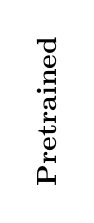
\begin{tikzpicture}
            \node[rotate=90] at (0, 0) {
                \textbf{Pretrained}
            };
        \end{tikzpicture}
    \end{minipage}%
    \hspace{1em}%
    \begin{minipage}{0.30\linewidth}
        \begin{centering}
            \scriptsize
            \textbf{Aesthetic Quality (New Animals)} \\
            \vspace{0.5em}
        \end{centering}
        \lfbox[
            border-width=2pt,
            padding-top=0pt,
            padding-bottom=0pt,
            padding-left=-2.5pt,
            padding-right=-4.8pt,
        ]{
            \begin{minipage}{\linewidth}
                \includegraphics*[width=0.5\linewidth]{generalization/before/flamingo.jpg}
                \hspace{-0.7em}
                \includegraphics*[width=0.5\linewidth]{generalization/before/starfish.jpg}
            \end{minipage}
        }
    \end{minipage}
    \hspace{0.5em}%
    \begin{minipage}{0.30\linewidth}
        \begin{centering}
            \scriptsize
            \textbf{Aesthetic Quality (Non-Animals)} \\
            \vspace{0.5em}
        \end{centering}
        \lfbox[
            border-width=2pt,
            padding-top=0pt,
            padding-bottom=0pt,
            padding-left=-2.5pt,
            padding-right=-4.8pt,
        ]{
            \begin{minipage}{\linewidth}
                \includegraphics*[width=0.5\linewidth]{generalization/before/bike.jpg}
                \hspace{-0.7em}
                \includegraphics*[width=0.5\linewidth]{generalization/before/fridge.jpg}
            \end{minipage}
        }
    \end{minipage}
    \hspace{0.5em}%
    \begin{minipage}{0.30\linewidth}
        \begin{centering}
            \scriptsize
            \textbf{Prompt Alignment (New Scenarios)} \\
            \vspace{0.5em}
        \end{centering}
        \lfbox[
            border-width=2pt,
            padding-top=0pt,
            padding-bottom=0pt,
            padding-left=-2.5pt,
            padding-right=-4.8pt,
        ]{
            \begin{minipage}{\linewidth}
                \includegraphics*[width=0.5\linewidth]{vlm/generalization/capybara_dishes_before.jpg}
                \hspace{-0.7em}
                \includegraphics*[width=0.5\linewidth]{vlm/duck_exam/0.jpg}
            \end{minipage}
        }
    \end{minipage}\\[0.1em]%
    \begin{minipage}{0.1em}
        \centering
        \scriptsize
        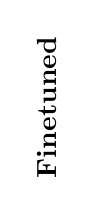
\begin{tikzpicture}
            \node[rotate=90] at (0, 0) {
                \textbf{Finetuned}
            };
        \end{tikzpicture}
    \end{minipage}%
    \hspace{1em}%
    \begin{minipage}{0.30\linewidth}
        \lfbox[
            border-width=2pt,
            padding-top=0pt,
            padding-bottom=0pt,
            padding-left=-2.5pt,
            padding-right=-4.8pt,
        ]{
            \begin{minipage}{\linewidth}
                \includegraphics*[width=0.5\linewidth]{generalization/flamingo.jpg}
                \hspace{-0.7em}
                \includegraphics*[width=0.5\linewidth]{generalization/starfish.jpg}
            \end{minipage}
        }
    \end{minipage}
    \hspace{0.5em}%
    \begin{minipage}{0.30\linewidth}
        \lfbox[
            border-width=2pt,
            padding-top=0pt,
            padding-bottom=0pt,
            padding-left=-2.5pt,
            padding-right=-4.8pt,
        ]{
            \begin{minipage}{\linewidth}
                \includegraphics*[width=0.5\linewidth]{generalization/bike.jpg}
                \hspace{-0.7em}
                \includegraphics*[width=0.5\linewidth]{generalization/fridge.jpg}
            \end{minipage}
        }
    \end{minipage}
    \hspace{0.5em}%
    \begin{minipage}{0.30\linewidth}
        \lfbox[
            border-width=2pt,
            padding-top=0pt,
            padding-bottom=0pt,
            padding-left=-2.5pt,
            padding-right=-4.8pt,
        ]{
            \begin{minipage}{\linewidth}
                \includegraphics*[width=0.5\linewidth]{vlm/generalization/capybara_dishes.jpg}
                \hspace{-0.7em}
                \includegraphics*[width=0.5\linewidth]{vlm/duck_exam/2.jpg}
            \end{minipage}
        }
    \end{minipage}%
    \caption{
        \textbf{(Generalization)}
        Finetuning on a limited set of animals generalizes to both new animals and non-animal everyday objects.
        The prompts for the rightmost two columns are ``\emph{a capybara washing dishes}'' and ``\emph{a duck taking an exam}''.
        A quantitative analysis is provided in Appendix~\ref{app:generalization}, and more samples are provided in Appendix~\ref{app:more_samples}.
    }
    \label{fig:generalization}
    \vspace{-15pt}
\end{figure}

\subsection{Generalization}
\label{sec:generalization}

RL finetuning on large language models has been shown to produce interesting generalization properties; for example, instruction finetuning almost entirely in English has been shown to improve capabilities in other languages \citep{ouyang2022instructgpt}.
It is difficult to reconcile this phenomenon with our current understanding of generalization; it would \emph{a priori} seem more likely for finetuning to have an effect only on the finetuning prompt set or distribution.
In order to investigate the same phenomenon with diffusion models, Figure~\ref{fig:generalization} shows a set of \methodours{}-finetuned model samples corresponding to prompts that were not seen during finetuning.
In concordance with instruction-following transfer in language modeling, we find that the effects of finetuning do generalize, even with prompt distributions as narrow as 45 animals and 3 activities.
We find evidence of generalization to animals outside of the training distribution, to non-animal everyday objects, and in the case of prompt-image alignment, even to novel activities such as ``\emph{taking an exam}''.











